\clearpage
\section{Point to Point Testinfrastruktur}\label{sec:PointtoPointTestinfrastruktur}

Im Nachfolgenden Abschnitt wird auf die Point to Point (P2P) Messung eingegangen. Ziel ist es die Verbindung auf MAC-Layer auszumessen und die aus Abschnitt ... aufgelisteten Messdaten zu erfassen. Dazu wird im folgenden auf das Messkonzept, den Messablauf und technische Einzelheiten eingegangen. 

\subsection{Konzept}\label{sec:KonzeptP2P}

Zur Realisierung der Point to Point Testinfrastruktur wurde auf eine \textit{One to Many} (1:n) Messprinzip gesetzt (auch als Broadcasting bekannt). Dies hat den Vorteil das mehrere Verbindungen gleichzeitig ausgemessen werden können. Der Nachteil dabei ist, dass die Messpfade nur unidirektional charakterisiert werden (nur von Master zu Slave oder Uplink-Pfad). Die Abweichung zwischen Up- und Downlink Pfad können durch wiederholen der Messung mit vertauschten Standorten verifiziert werden. 

\begin{figure} [H]
	\centering
	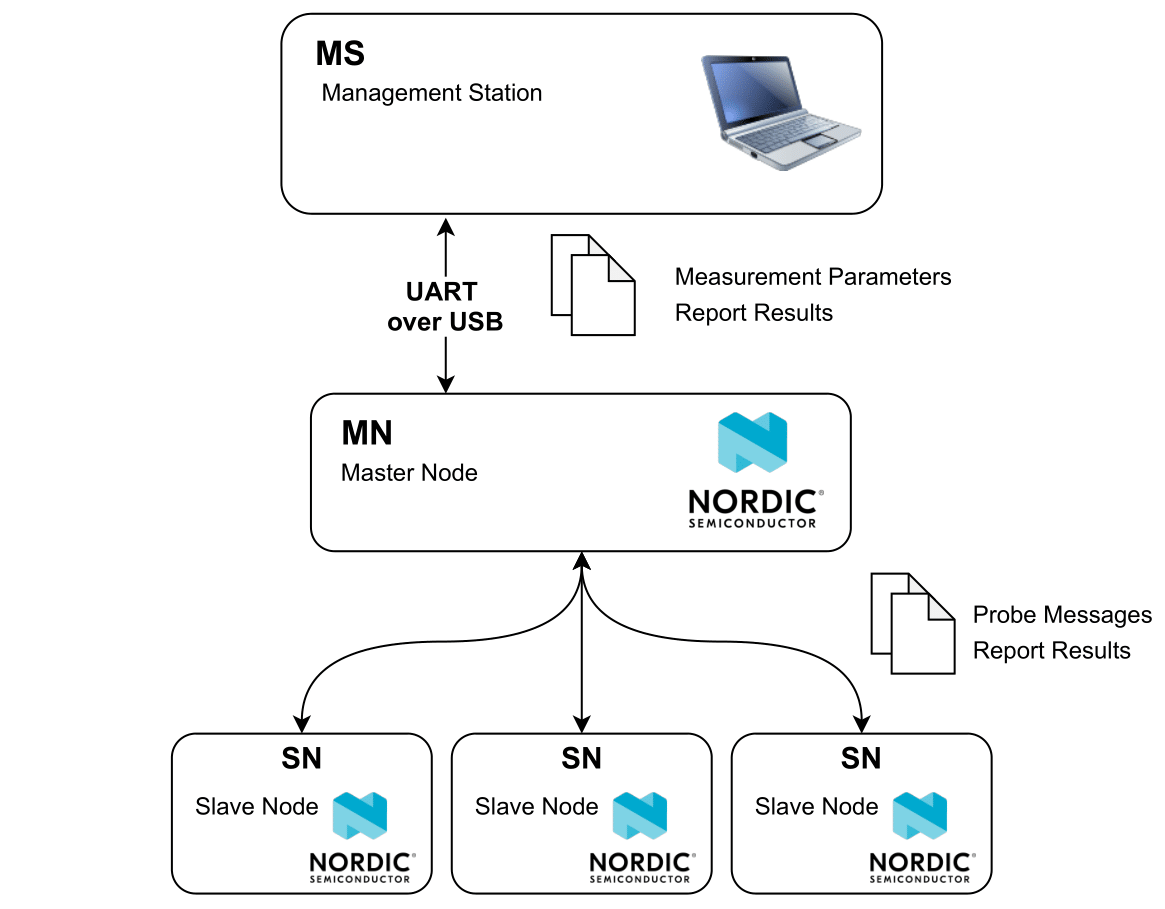
\includegraphics[width=0.8\textwidth]{Konzeptschema_P2P.png}
	\caption{Konzeptschema P2P Testinfrastruktur}
	\label{fig:KonzeptschemaP2P}
\end{figure}

Das in Abbildung \ref{fig:KonzeptschemaP2P} gezeigte Konzept besteht aus einer Managment Station, einem Master- und mehreren Slave Nodes. Über die Management Station können Messresultate angezeigt, sowie Messparameter eingestellt werden. Als Ausgangspunkt zur Messung dient der MN (Master Node). Er koordiniert den Messablauf und sendet \textit{Probe Packets} an alle SN (Slave Nodes). Diese Protokollieren die Anzahl empfangener \textit{Probe Packets} und melden ihre Messresultate an den MN zurück. Nach Empfang aller Resultate leitet der MN alle Messergebnisse an die MS weiter. Dort werden dem Benutzer die Messdaten dargestellt. Details zum Ablauf sind in Abschnitt \ref{sec:SoftundFirmware} aufgeführt. Eine mögliche Anwendung der Testinfrastruktur wird im folgenden Abschnitt \ref{sec:TestszenarienP2P} beschrieben.  

\subsection{Testszenarien}\label{sec:TestszenarienP2P}

Die P2P Testinfrastruktur ist als einfach zu bedienendes Tool konzipiert. Es kann eingesetzt werden um den Aufbau von 

\todo[inline]{Testumgebungen sowie die Beziehungen der Knoten innerhalb der Point to Point Messung beschreiben.}

\subsection{Ablauf}\label{sec:AblaufP2P}
\todo[inline]{Ablauf eines Point to Point MAC Layer Benchmarks aus Anwendersicht beschreiben.}

\subsection{Messgrössen}\label{sec:MessgrössenP2P}
\todo[inline]{Erläuterung der Messgrössen die erfasst werden sollen. Inkl. Beschreibung wie dies technisch umgesetzt wird.}

\subsection{Messaufbau}\label{sec:Messaufbau}
\todo[inline]{Schema inkl. Beschreibung.}

\subsection{Aufbau und Bedienung der Messinfrastruktur}\label{sec:AufbauundBedienungderMessinfrastruktur}
\todo[inline]{Bedienungsanleitung des Messaufbaus.}

\subsection{Interpretation der Messresultate für den Anwender}\label{sec:InterpretationderMessresultatefürdenAnwender}
\todo[inline]{Wie sind die Resultate zu interpretieren. Welche Schlüsse können/müssen aus den Resultaten gezogen werden. Welche Resultate bedeuten was?}

\subsection{Soft- und Firmware}\label{sec:SoftundFirmware}
\todo[inline]{Beschreibung der Node-Firmware sowie der Auswertesoftware auf dem Raspi.}




\subsection{Zeitsynchronisation}\label{sec:Zeitsynchronisation}
\todo[inline]{Wie wurde die Zeitsynchronisation umgesetzt? Wie relevant ist diese für die Messungen?}